\documentclass[conference]{IEEEtran}
\usepackage[utf8]{inputenc}
\IEEEoverridecommandlockouts
% The preceding line is only needed to identify funding in the first footnote. If that is unneeded, please comment it out.
\usepackage{cite}
\usepackage{float}
\usepackage{amsmath,amssymb,amsfonts}
\usepackage{algorithmic}
\usepackage{graphicx}
\usepackage{textcomp}
\usepackage{xcolor}
\usepackage{hyperref}
\usepackage{ngerman}
\def\BibTeX{{\rm B\kern-.05em{\sc i\kern-.025em b}\kern-.08em
    T\kern-.1667em\lower.7ex\hbox{E}\kern-.125emX}}
\begin{document}

\title{Konzeptpapier\\Bomberman?}

% Authoren	
\author{
	\IEEEauthorblockN{Bösl, Florian}
	\IEEEauthorblockA{
		\textit{f.boesl@oth-aw.de}\\
	}
	\and

	\IEEEauthorblockN{Chernysheva Anastasia}
	\IEEEauthorblockA{
		\textit{a.chernysheva@oth-aw.de}\\
	}
	\and

	\IEEEauthorblockN{Kohl Helge}
	\IEEEauthorblockA{
		\textit{h.kohl@oth-aw.de}\\
	}
	\and

	\IEEEauthorblockN{Korinth Patrice}
	\IEEEauthorblockA{
		\textit{p.korinth@oth-aw.de}\\
	}
	\and

	\IEEEauthorblockN{Porsch Philipp}
	\IEEEauthorblockA{
		\textit{p.porsch@oth-aw.de}\\
	}
}

\maketitle

\begin{abstract}
	Online-Spiele erfreuen sich coronabedingt immer größerer Beliebtheit. Dies könnte vor allem aus der unkomplizierten Zugangsmöglichkeit der Online-Spiele resultieren, aber auch der sich als redundant erweisenden Softwareinstallation. Die 
	Online-Spiele wurden damals mit der Adobe Software 'Flash' realisiert. Aufgrund der Risiken auf der Sicherheitsebene wurde die Unterstützung der Software eingestellt. Heutzutage bedient man sich verschiedener Webtechnologien, die im Kapitel IV näher beleuchtet werden.
	Darin begründet liegt die Motivation hinter dieser Arbeit, denn 
	die Spieleentwicklung ermöglicht eine intensive Auseinandersetzung mit diesen Webtechnologien, aber auch der Kreativität seinen freien Lauf zu lassen.
	Der Fokus dieser Arbeit liegt in der Entwicklung eines cloudbasiertes Online-Multiplayer-Spiels. Als Inspiration dient an erster Stelle der zeitlose Klassiker "Bomberman".
\end{abstract}

\section{Einführung}
Bereits 1983 kam das labyrinthartig aufgebaute Computerspiel "Bomberman", das vom japanischen Hersteller Hudson Soft (wurde 2012 von Konami übernommen) entwickelt wurde, auf den Markt. Seitdem erschienen bis heute zahlreiche, offizielle und daran angelehnte Spiele. Dabei hat sich das grundsätzliche Spielprinzip nie verändert. Das Spielfeld besteht aus zerstörbaren und unzerstörbaren Wänden. Strategisch legt der Spieler Bomben und bringt damit die zerstörbaren Wände zum Einsturz, um sich den Weg freizumachen. Durch die Zerstörung können versteckte Items in Erscheinung treten, die dem Spieler sehr nützlich sein können. Insbesondere der Multiplayer-Modus ist bei der Community sehr beliebt. Dieser verleitet dazu seine Mitspieler durch das Wegsprengen zu beseitigen. Ein Levelaufstieg finden statt, sobald alle Gegner exterminiert wurden.  



\section{Verwandte Arbeiten}
Nachdem in der Zusammenfassung bereits die Motivation erläutert wurde, werden hier verwandte Arbeiten und Systeme vorgestellt. Bei der Recherche wurden einige Bomberman inspirierte Online-Spiele gefunden, die auch kostenlos verfügbar sind. Spiel \cite{bombe-friends}, Bomber-Friends, stellt dabei eine komplexe Variante des Spiels dar, aufgrund von RPG-Elementen, die den klassischen Spielstil mit der Möglichkeit erweitert, aus zerstörten Boxen Edelsteine zu gewinnen, mit denen sich Verbesserungen freischalten lassen. Power-Ups sind ebenfalls erhältlich. 
\begin{figure}[H]
    \centering
    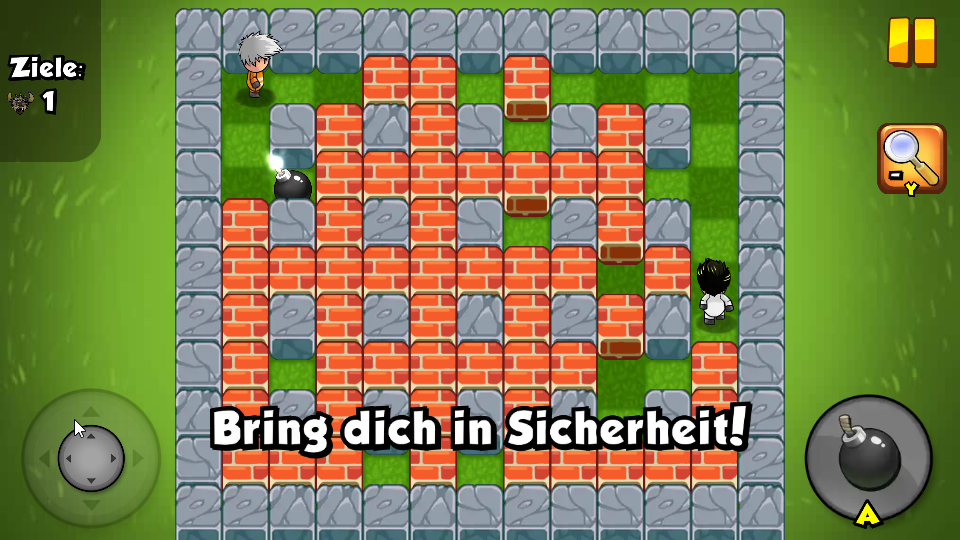
\includegraphics[width=0.45\textwidth]{res/bomberfriends.png}
    \caption{Bomber-Friends}
\end{figure}

Bomber-Mouse \cite{bombermouse} hingegen ist eine simplere Version, in der sich der Charakter nur sehr langsam fortbewegt, was möglicherweise nicht beabsichtigt ist. Auch die Fenstergröße passt sich nicht automatisch an und das Game Design weist allgemein deutliche Mängel auf.
\begin{figure}[H]
    \centering
    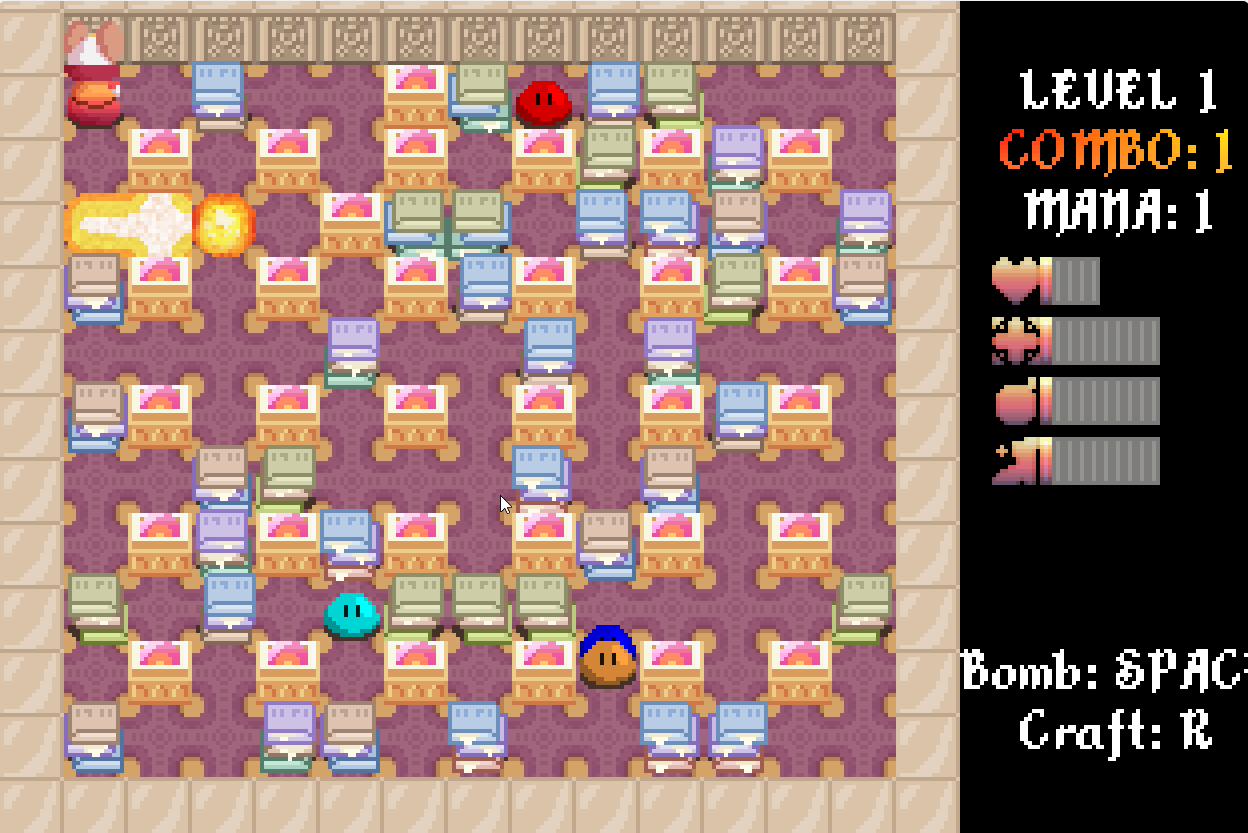
\includegraphics[width=0.45\textwidth]{res/bombermouse.png}
    \caption{Bomber Mouse}
\end{figure}
Playing with Fire 2 \cite{playingwithfire} weist die meisten Individualisierungsmöglichkeiten in der Lobby auf. So kann die Anzahl der Spieler und die der Gegner festgelegt werden sowie die Auswahl des Levels. Zusätzlich läuft ein Timer ab, der die Schwierigkeit erhöht. 
\begin{figure}[H]
    \centering
    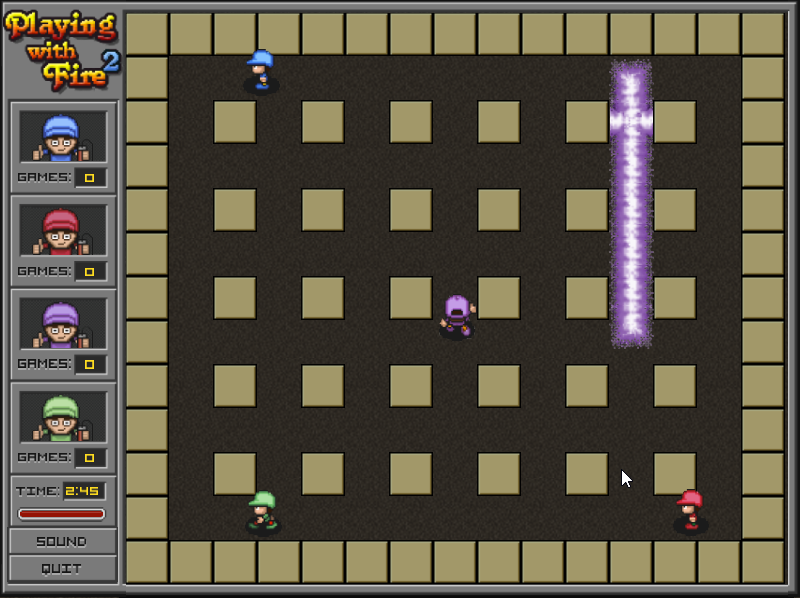
\includegraphics[width=0.45\textwidth]{res/playing-with-fire.png}
    \caption{Playing with Fire}
\end{figure}


Allstar-Blast \cite{allstarblast} ist eine MMO-Variante von Ubisoft, in der bis zu 100 Spieler gleichzeitig gegeneinander antreten. Die Besonderheit hierbei ist, dass das Spielfeld mit der Zeit schrumpft. Power-Ups sind hier ebenfalls verfügbar.
\begin{figure}[H]
    \centering
    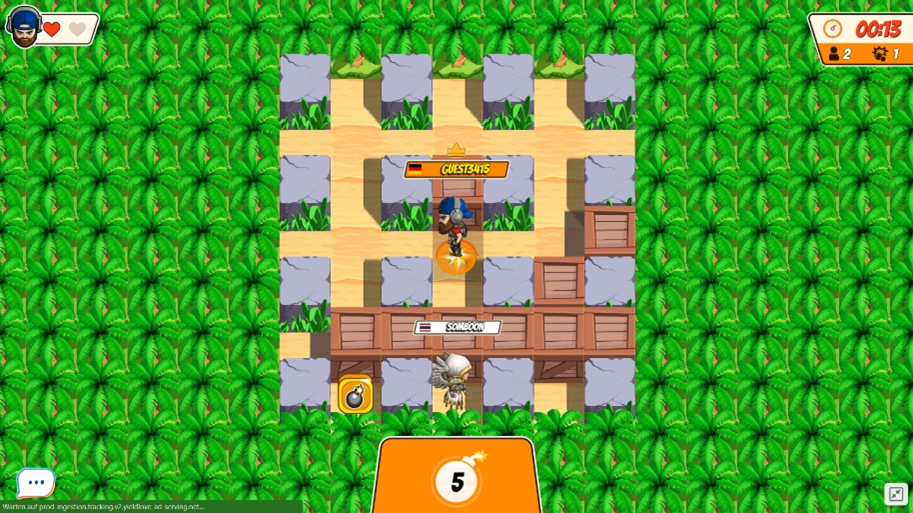
\includegraphics[width=0.45\textwidth]{res/all-star-blast.png}
    \caption{Allstar-Blast}
\end{figure}


\section{Anforderungen}

\subsection{Anforderung 1} (mvp)
Als Spieler möchte ich ein Spiel eröffnen können, um ein Spiel spielen zu können.

\subsection{Anforderung 2} (mvp)
Als Spieler möchte ich mich auf dem Spielfeld bewegen können, um mit der Umgebung zu interagieren.

\subsection{Anforderung 3} (mvp)
Als Spieler möchte ich Bomben legen können, damit sie später explodieren können.

\subsection{Anforderung 4} (mvp)
Als Spieler möchte ich, dass die Bomben explodieren und verschwinden, um ihren Effekt visuell zu erleben (und das Spiel zu gewinnen).

% next
\subsection{Anforderung 5} 
Als Spieler möchte ich mit Hindernissen kollidieren können, um Einschränkungen in der Spielwelt zu haben.

\subsection{Anforderung 6}
Als Spieler möchte ich, dass die Bomben bei ihrer Explosion Hindernisse zerstören, um die Spielwelt zu manipulieren.

\subsection{Anforderung 7} 
Als Spieler möchte ich einem Spiel beitreten können, um in einem bestehenden Spiel mitspielen zu können.

\subsection{Anforderung 8}
Als Spieler möchte ich, dass meine Spielfigur bei Kontakt mit anderen Spielfiguren kollidiert, um den Bewegungsspielraum des Gegners einzuschränken.

\subsection{Anforderung 9}
Als Spieler möchte ich, dass der Kontakt von Bombenexplosionen und Spielfiguren erkannt wird, um diese zu zerstören.

\subsection{Anforderung 10}
Als Spieler möchte ich, dass ich wenn der letzte Gegner besiegt ist, das Spiel beendet wird, um den Abschluss der Spielziels zu erkennen.

\subsection{Anforderung 11}
Als Spieler möchte ich jederzeit spielen können, um bei hohen Spielerzahlen keine Wartezeiten zu haben.

\subsection{Anforderung 12} 
Als Anbieter möchte ich, dass Spiele bei zu langer Spieldauer beendet werden, um Rechenkapazitäten zu sparen.

% bonus
\subsection{Anforderung 13}
Als Spieler möchte ich mit mehr als einem weiteren Spieler spielen können, um den Komplexitätsgrad des Spieles zu erhöhen.

\subsection{Anforderung 14}
Als Spieler möchte ich eine dynamische Spielfeldgröße, um den Umfang des Spiels zu erhöhen (nochmal drübernachdenken).

\subsection{Anforderung 15}
Als Spieler möchte ich meinen Spielernamen festlegen können, um einen Wiedererkennungswert zu schaffen.

\subsection{Anforderung 16}
Als Spieler möchte ich ein Leaderboard einsehen können, um meine Leistung kompetitiv einordnen zu können.

\subsection{Anforderung 17}
Als Spieler möchte ich meine Spielfigur personalisieren können, um meine Figur an meinen Geschmack anzupassen.

\subsection{Anforderung 18}
Als Spieler möchte ich Power-Ups einsammeln können, um das Spielerlebnis aufzuwerten.

\section{Methoden}
Die Spieldaten werden in einer Datenbank gespeichert. Diese beinhalten Informationen, beispielsweise zu den Spieleinstellungen, Gegnern, Spielstatus oder das Inventar der Spielers. 
Die Verwaltung der Spieldaten und Logik soll im Hintergrund über einen oder mehrere Amazon S3 Buckets geregelt werden und dadurch auch eine Skalierbarkeit ermöglichen. Wird ein neues Spiel eröffnet, so kann beispielsweise dafür ein neuer Bucket initialisiert werden. Eine Alternative dazu wäre das Erstellen von Docker-Containern, da diese auf jeder Hardware umsetzbar sind und auf Anfrage weitere davon zugeschaltet werden könnten. Die Umgebung innerhalb des Servers wird mit NodeJS umgesetzt werden, da dies das Bereitstellen von Dateien und Websockets für die User ermöglicht. 
Die Game Engine, die der Nutzer zu sehen bekommen wird mit HTML5 implementiert. Des Weiteren wird das Framework 'Phaser' verwendet, um dem Nutzer grafische Ausgaben zu liefern und die Eingaben des Nutzers an das Spiel zu verarbeiten.
Da Cheating ein große Problematik, insbesondere beim Multiplayer-Spiel, darstellt, werden alle empfangenen Daten auf dem Server validiert. Dies löst zwar das Problem nicht vollständig, sollte jedoch kleine Angriffe abwehren. 
\begin{figure}[H]
    \centering
    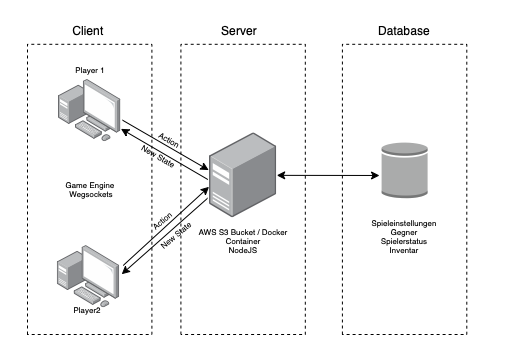
\includegraphics[width=0.5\textwidth]{res/game_arch.png}
    \caption{Spiel Architektur}
\end{figure}

\section{Graphischer Prototyp}
Die grafische Oberfläche des Spiels teilt sich in zwei verschiedene Bereiche auf. Im oberen Fenster befinden sich aktuelle Informationen zum Spiel. So wird Name und das Avatarbild des Spielers und des Mitspielers angezeigt, sowie die Anzahl der, sich im Inventar befindenden, Bomben. Das Spielfeld nimmt den restlichen Platz ein. Das Spielfeld besteht aus folgenden Spielelementen: zerstörbare und unzerstörbare Wände, die sich optisch voneinander unterschieden. Damit wird dem Spieler die Differenzierung zwischen beiden visuell ermöglicht. Des Weiteren kommen zwei Arten von Gegnern vor: der Mitspieler sowie die vom Spiel generierten Enemys. Die Elementen mit der höchsten Relevanz sind jedoch der Spieler selbst sowie die Bomben. Weitere Bestandteile, die nicht in der Abbildung 6 dargestellt wurden, sind: Items aus der Wandzerstörung, sowie Spielmenü-Elemente. 
\begin{figure}[H]
    \centering
    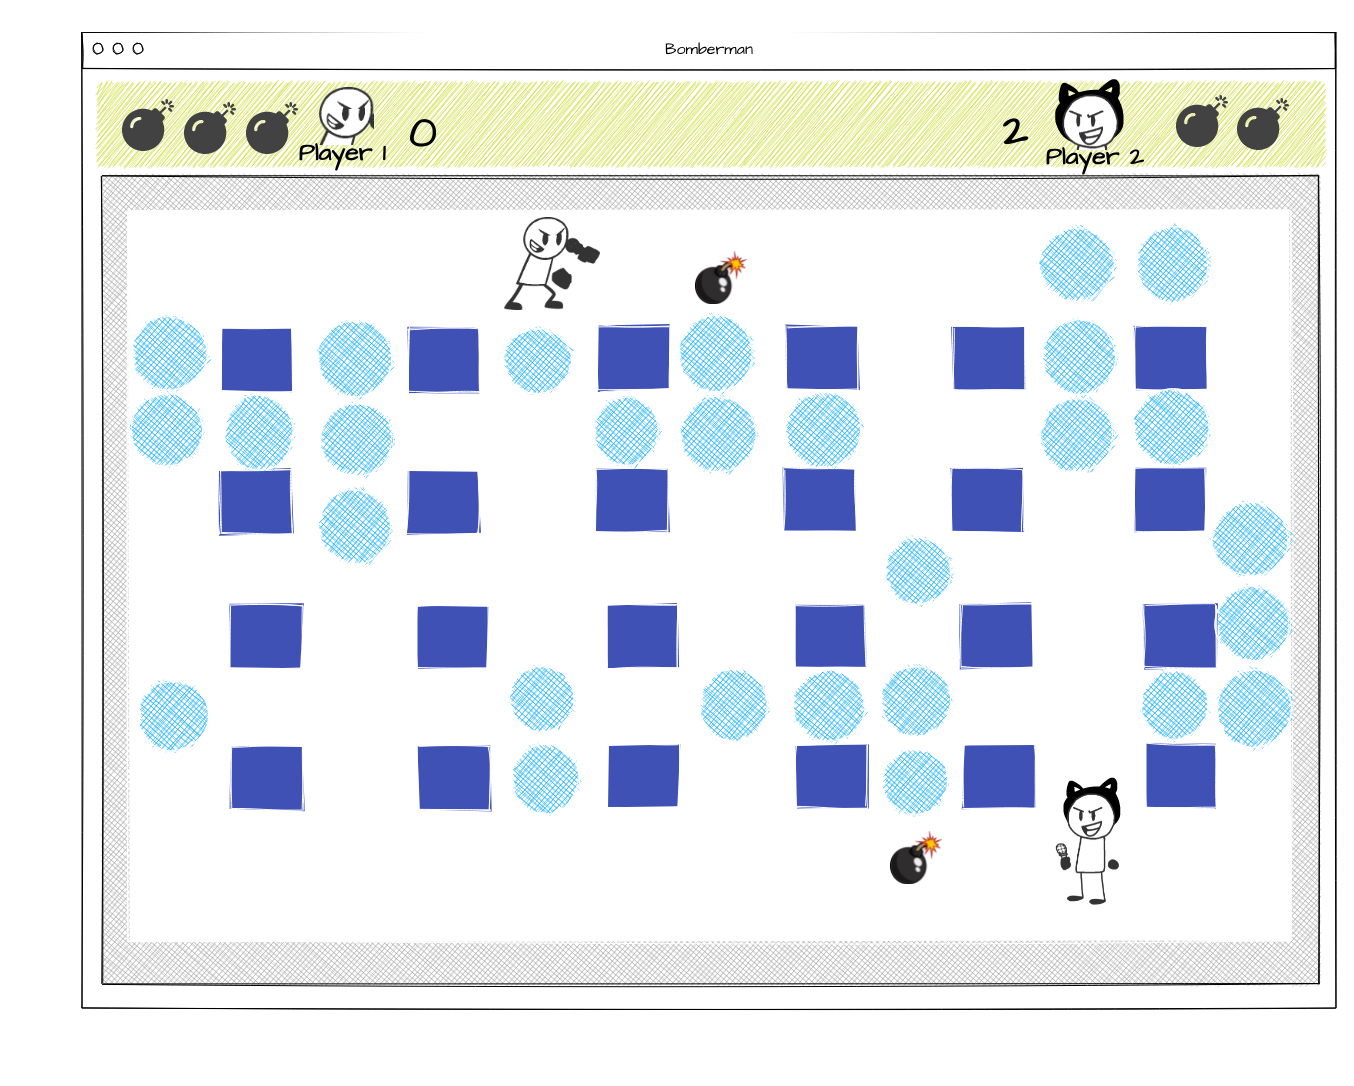
\includegraphics[width=0.5\textwidth]{res/prototyp.png}
    \caption{Prototyp des Spiels}
\end{figure}
%\section*{Referenzen}

\nocite{space-invaders}
\begin{thebibliography}{0}
	\bibitem{bombe-friends}Bomber-Friends [Online] \url{https://www.spielaffe.de/Spiel/Bomber-Friends} (visited on May. 03, 2022)
	\bibitem{bombermouse}Bomber-Mouse [Online] \url{https://de.y8.com/games/bomber_mouse} (visited on May. 03, 2022)
	\bibitem{playingwithfire}Playing-with-Fire [Online] \url{https://www.kibagames.com/Game/Playing-with-Fire-2 } (visited on May. 03, 2022)
	\bibitem{allstarblast}Allstar-blast [Online] \url{https://www.kibagames.com/Game/All-Star-Blast} (visited on May. 03, 2022)
	\bibitem{space-invaders}S. Neelakantam,	\textit{Building a realtime multiplayer browser game in less than a day} [Online] \url{https://medium.com/@n.srushtika/building-a-realtime-multiplayer-browser-game-in-less-than-a-day-part-1-4-4ff35dd44715} (visited on May. 06, 2022)

\end{thebibliography}
\vspace{12pt}

\end{document}
